\chapter{Description du Parcours}

Mon parcours professionnel s'articule autour d'une progression cohérente qui m'a conduit de l'expertise technique industrielle vers l'enseignement supérieur, en passant par une reconversion maîtrisée vers l'Éducation Nationale. Cette trajectoire de près de 25 ans révèle une constante : l'adaptation permanente aux évolutions technologiques et la transmission de savoirs, d'abord en entreprise puis en établissement scolaire.

La solidité de ma formation initiale en informatique, acquise à l'IUT du Havre puis complétée par de nombreuses certifications professionnelles, a constitué le socle d'une carrière industrielle de 15 ans dans des environnements techniques exigeants. Cette expertise approfondie des systèmes, réseaux et développement logiciel correspond aux modules techniques du Master MEEF Informatique \parencite{master_meef_nantes}, couvrant notamment la programmation, l'algorithmique, l'architecture des ordinateurs et les réseaux.

L'évolution vers des responsabilités managériales, culminant avec 11 années de team leadership chez SopraStéria, a développé mes compétences en gestion d'équipes, formation de collaborateurs et communication avec des publics variés. Ces compétences transversales \parencite{competences_transversales} trouvent leur prolongement naturel dans les compétences du référentiel MEEF centrées sur la pratique réflexive et l'analyse de l'activité pédagogique \parencite{referentiel_meef}.

\section{Frise chronologique du parcours}

\begin{center}
    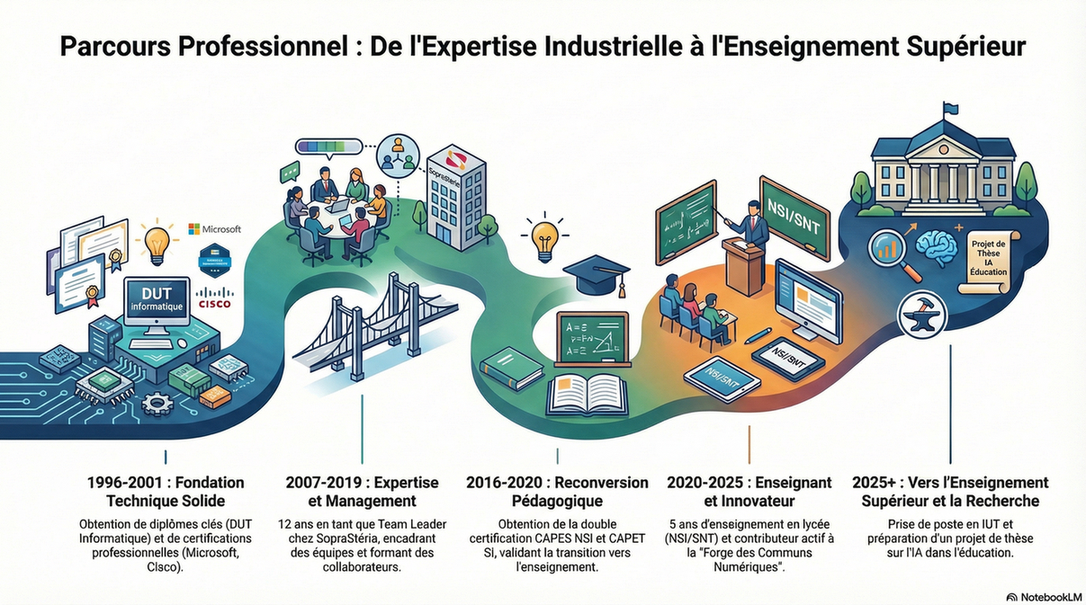
\includegraphics[width=\textwidth]{sources/medias/parcours.png}
    \\ \vspace{0.5cm} \small \textit{Illustration réalisée avec NotebookLM}
\end{center}

\section{Temps forts et correspondances avec le référentiel MEEF}

\subsection{Phase 1 : Formation technique solide (1996-2001)}

Ma formation initiale révèle une progression logique vers l'expertise informatique. Le DUT Informatique Génie Logiciel obtenu à l'IUT du Havre en 1999 m'a apporté les fondamentaux de la programmation et de l'algorithmique, compétences directement transférables aux enseignements techniques du Master MEEF \parencite{master_meef_nantes}. Les certifications Microsoft (MCSE, MCP) et CISCO (CCNA) acquises en autoformation en 2000 témoignent d'une capacité d'apprentissage autonome et d'une veille technologique constante, qualités essentielles pour la formation à et par la recherche \parencite{referentiel_meef}.

\subsection{Phase 2 : Expertise professionnelle et management (2004-2019)}

Mes 15 années d'expérience industrielle couvrent l'ensemble du spectre technique du Master MEEF Informatique. En tant que responsable SAV chez Nicolas et Fils (2004-2006), j'ai développé des compétences en relation client et résolution de problèmes complexes. Mon passage chez TOTAL/CPI (2006-2007) comme développeur d'applications métiers correspond aux UE de programmation avancée et bases de données.

L'évolution vers team leader chez TOTAL/Stéria puis SopraStéria (2007-2019) a développé mes compétences managériales et pédagogiques. Former des collaborateurs, animer des équipes techniques et communiquer avec des interlocuteurs variés constituent autant de compétences transférables vers l'enseignement \parencite{knowles_andragogy}, particulièrement pour les aspects centrés sur la pratique réflexive \parencite{schon_reflective_practitioner}.

\subsection{Phase 3 : Reconversion maîtrisée (2016-2020)}

La formation « Concepteur Architecte en Ingénierie de Projets » suivie en contrat de professionnalisation (2016-2018) illustre ma capacité à me former en parallèle de mon activité professionnelle. Cette démarche préfigure l'approche recherche attendue dans le Master MEEF. L'obtention simultanée du CAPES NSI et du CAPET SI en 2020 \parencite{capes_nsi} témoigne d'une reconversion préparée et d'une double compétence valorisante pour l'enseignement technologique et scientifique.

\subsection{Phase 4 : Développement pédagogique (2020-2025)}

Mes cinq années d'enseignement en lycée (SNT/NSI) correspondent à une mise en pratique progressive des compétences pédagogiques conformément aux programmes officiels \parencite{eduscol_nsi,baccalaureat_nsi}. La participation régulière aux formations académiques (évaluation, programmation fonctionnelle, gestes inclusifs) révèle un engagement dans la formation continue conforme aux exigences du Master MEEF \parencite{referentiel_meef}. L'évolution vers l'IUT en 2025 pour enseigner les « Ressources et Culture Numérique » \parencite{but_informatique} marque une progression naturelle vers l'enseignement supérieur.

\section{Tableaux de correspondance avec le référentiel MEEF}

L'analyse détaillée des correspondances entre mon parcours professionnel et les modules du Master MEEF Informatique est présentée dans le \textbf{Chapitre 12 - Synthèse de la correspondance}, section \textbf{12.1 Tableau récapitulatif de couverture des blocs de compétences}.

Cette synthèse démontre la couverture exhaustive des compétences attendues du référentiel RNCP38152 par mon expérience industrielle, managériale et pédagogique.

\section{Cohérence du parcours et perspectives}

Cette description révèle un parcours cohérent où chaque étape prépare la suivante. L'expertise technique acquise en 20 ans d'industrie légitime mon enseignement des disciplines informatiques. L'expérience managériale développe les compétences relationnelles et pédagogiques \parencite{competences_transversales}. La reconversion vers l'enseignement s'appuie sur une certification solide (CAPES/CAPET) et une pratique de terrain de 5 ans.

L'évolution actuelle vers l'IUT et le projet de thèse sur l'impact de l'intelligence artificielle dans l'éducation \parencite{intelligence_artificielle_education} s'inscrivent naturellement dans cette progression. Mon parcours illustre la complémentarité entre expertise disciplinaire, compétences pédagogiques et démarche de recherche attendues dans le Master MEEF Pratiques et Ingénierie de la Formation (PIF) \parencite{rncp38152,referentiel_meef}.

Cette trajectoire professionnelle, de l'industrie vers l'enseignement supérieur, constitue un atout majeur pour former les futurs enseignants d'informatique en leur apportant une vision concrète des enjeux professionnels et technologiques de la discipline.